\documentclass{article}
\usepackage{ctex, hyperref}
%\usepackage[utf8]{inputenc}
\usepackage[top=2cm, bottom=2cm, left=2cm, right=2cm]{geometry}  
\usepackage{algorithm}  
\usepackage{algpseudocode}  
\usepackage{amsmath}
\usepackage{float}  
\usepackage{multirow}

\usepackage{listings} 
\usepackage{xcolor}
\definecolor{mygreen}{rgb}{0,0.6,0}  
\definecolor{mygray}{rgb}{0.5,0.5,0.5}  
\definecolor{mymauve}{rgb}{0.58,0,0.82}  
  
\lstset{ %  
  backgroundcolor=\color{white},   % choose the background color; you must add \usepackage{color} or \usepackage{xcolor}  
  basicstyle=\footnotesize,        % the size of the fonts that are used for the code  
  breakatwhitespace=false,         % sets if automatic breaks should only happen at whitespace  
  breaklines=true,                 % sets automatic line breaking  
  captionpos=bl,                    % sets the caption-position to bottom  
  commentstyle=\color{mygreen},    % comment style  
  deletekeywords={...},            % if you want to delete keywords from the given language  
  escapeinside={\%*}{*)},          % if you want to add LaTeX within your code  
  extendedchars=true,              % lets you use non-ASCII characters; for 8-bits encodings only, does not work with UTF-8  
  frame=single,                    % adds a frame around the code  
  keepspaces=true,                 % keeps spaces in text, useful for keeping indentation of code (possibly needs columns=flexible)  
  keywordstyle=\color{blue},       % keyword style  
  %language=Python,                 % the language of the code  
  morekeywords={*,...},            % if you want to add more keywords to the set  
  numbers=left,                    % where to put the line-numbers; possible values are (none, left, right)  
  numbersep=5pt,                   % how far the line-numbers are from the code  
  numberstyle=\tiny\color{mygray}, % the style that is used for the line-numbers  
  rulecolor=\color{black},         % if not set, the frame-color may be changed on line-breaks within not-black text (e.g. comments (green here))  
  showspaces=false,                % show spaces everywhere adding particular underscores; it overrides 'showstringspaces'  
  showstringspaces=false,          % underline spaces within strings only  
  showtabs=false,                  % show tabs within strings adding particular underscores  
  stepnumber=1,                    % the step between two line-numbers. If it's 1, each line will be numbered  
  stringstyle=\color{orange},     % string literal style  
  tabsize=2,                       % sets default tabsize to 2 spaces  
  %title=myPython.py                   % show the filename of files included with \lstinputlisting; also try caption instead of title  
} 


\floatname{algorithm}{algorithm}  
\renewcommand{\algorithmicrequire}{\textbf{Input:}}
\renewcommand{\algorithmicensure}{\textbf{Output:}}

\usepackage{graphicx}

\usepackage[english]{isodate}

\title{\Huge \textbf {微分方程数值解 (第九章理论作业)} }
\author{褚朱钇恒 - 3200104144}


\begin{document}

\maketitle

\section{Exercise 9.5}
$Ae = r \Rightarrow ||Ae||_2=||r||_2\le ||A||_2||e||_2$


$Ax = b \Rightarrow x = A^{-1}b \Rightarrow ||A^{-1}b||_2=||x||_2\le ||A^{-1}||_2||b||_2$ 且 $||Ax||_2=||b||_2\le ||A||_2||x||_2$

$Cond(A)\frac{||r||_2}{||b||_2}=\frac{||A||_2||A^{-1}||_2||r||_2}{||b||_2}\ge \frac{||A||_2||A^{-1}r||_2}{||A||_2||x||_2}=\frac{||e||_2}{||x||_2}$

$\frac{||r||_2}{Cond(A)||b||_2}= \frac{||r||_2}{||A||_2||A^{-1}||_2||b||_2} \le \frac{||A||_2||x||_2}{||A||_2||e||_2} =\frac{||e||_2}{||x||_2}$

\section{Exercise 9.8}
由于A对称,则有
$||A||_2=\sqrt[]{\lambda_{max}(A^TA)}=|\lambda_{max}(A)|$

同理$||A^{-1}||_2=\frac{1}{|\lambda_{min}(A)|}$

故有$cond(A)=\frac{|\lambda_{max}(A)|}{|\lambda_{min}(A)|}$

$n=8$时,$cond(A)=\frac{|\lambda_{max}(A)|}{|\lambda_{min}(A)|}=\frac{\frac{4}{h^2}sin^2\frac{k_{max}\pi}{2(m+1)}}{\frac{4}{h^2}sin^2\frac{k_{min}\pi}{2(m+1)}}=\frac{sin^2\frac{7\pi}{16}}{sin^2\frac{\pi}{16}}$

同理$n=1024$时,$cond(A)=\frac{|\lambda_{max}(A)|}{|\lambda_{min}(A)|}=\frac{\frac{4}{h^2}sin^2\frac{k_{max}\pi}{2(m+1)}}{\frac{4}{h^2}sin^2\frac{k_{min}\pi}{2(m+1)}}=\frac{sin^2\frac{1023\pi}{2048}}{sin^2\frac{\pi}{2048}}$

\section{Exercise 9.14}
可以发现,以下两条图像在$\frac{i}{n}$处相交,所以在$\Omega=(0,1)$的$h=\frac{1}{6}$的网格上无法区分两者。
\begin{figure}[H]
    \centering
    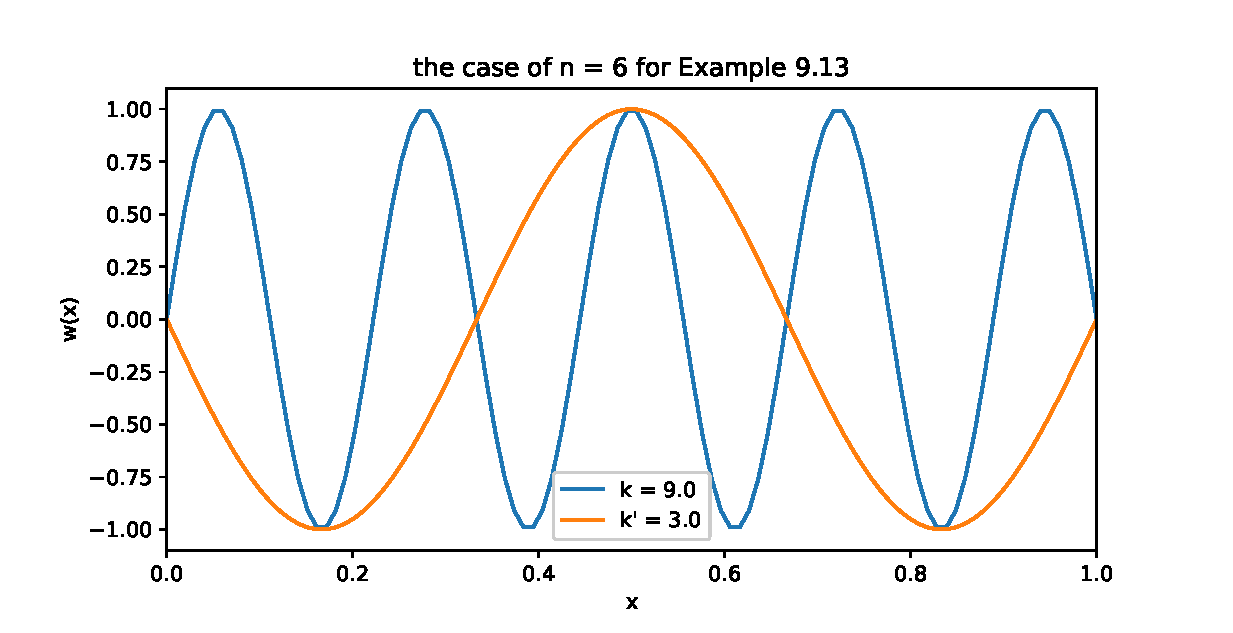
\includegraphics[width=10cm]{./9_14.eps}
\end{figure}

\section{Exercise 9.17}
由$\lambda(A)=\frac{4}{h^2}sin^2\frac{k\pi}{2(m+1)}$,设其特征向量为$x_k$,则有

$T_\omega x_k=Ix_k-\frac{\omega h^2}{2}Ax_k=x_k-2\omega sin^2\frac{k\pi}{2n}x_k$,故有

$\lambda(T_\omega)=1-2\omega sin^2\frac{k\pi}{2n}$

\section{Exercise 9.35}

当$v_1=v_2=1$,FMG的时间复杂度为$\Sigma_{i=0}^m2^{-iDm}\Sigma_{i=0}^m2^{-iDm}2WD=\frac{2}{(1-2^{-D})^2}WU$

将$D=1,2,3$代入则可得到上界分别为$8WU,\frac{32}{9}WU,\frac{128}{49}WU$

\section{Exercise 9.45}

$N(I_h^{2h})=\{v^h \in \Omega^h\ and \ v^h_{2*i+1}=-(v^h_{2*i}+v^h_{2*i+2})\}$

所以$\dim N(I_h^{2h})=\frac{n}{2}$

由于$I^h_{2h}$与$I_h^{2h}$互为逆变换,则$\dim R(I^h_{2h})=\dim R(I_h^{2h})=\frac{n}{2}-1$
\end{document}


